\documentclass[main.tex]{subfiles}

\begin{document}

%-------------------------------------------------------------------------------
%-------------------------------- Subsection 1.7 -------------------------------
%-------------------------------------------------------------------------------
\subsection{Integrálok összefoglaló}


\begin{figure}[H]
  \centering
  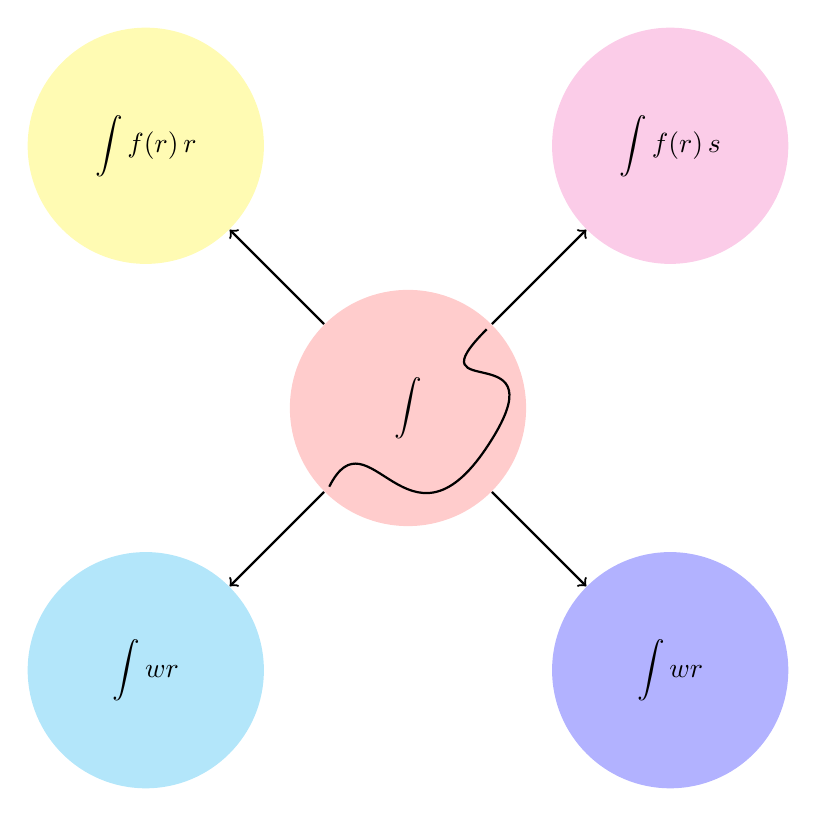
\begin{tikzpicture}
    \pgfmathsetmacro{\ra}{3.33}

    \node [circle, fill=red!20, minimum size=3cm] (O) at (0, 0) {
      $\displaystyle\int$
    };
    \draw [thick]  (-1, -1) .. controls (-.5,0) and (0,-2) .. (1,-.5);
    \draw [thick]   (1,-.5) .. controls (2,1) and (0, 0) .. (1,1);


    \node [circle, fill=magenta!20, minimum size=3cm] (A) at (\ra, \ra) {
      $\displaystyle\int f(\rvec{r}) \, \differential s$
    };

    \node [circle, fill=blue!30, minimum size=3cm] (B) at (\ra, -\ra) {
      $\displaystyle\int \scalar{\rvec{w}}{\differential\rvec{r}}$
    };

    \node [circle, fill=cyan!30, minimum size=3cm] (C) at (-\ra, -\ra) {
      $\displaystyle\int \rvec{w} \cross \differential \rvec{r}$
    };

    \node [circle, fill=yellow!30, minimum size=3cm] (D) at (-\ra, \ra) {
      $\displaystyle\int f(\rvec{r}) \, \differential \rvec{r}$
    };

    \foreach \i/\j in {A/right, B/right, C/left, D/left}{
        \draw [thick, ->] (O) -- (\i);
        % \node [
        %   thick,
        %   rectangle,
        %   \j=2.5cm,
        %   fill=yellow!10,
        %   draw=black,
        %   minimum width=2.5cm,
        %   minimum height=3cm,
        %   rounded corners=3px
        % ] at (\i) {};
      }

  \end{tikzpicture}
  \caption{Görbe menti integrálok}
\end{figure}

\begin{figure}[H]
  \centering
  \begin{tikzpicture}[
      declare function={f(\x,\y)=exp(-\x^2-\y^2);}
    ]
    \pgfmathsetmacro{\ra}{3.33}

    \node [circle, fill=red!20, minimum size=3cm] (O) at (0, 0) {};

    \begin{scope}[
        xshift=-1.1cm,
        yshift=-1.2cm
      ]
      \begin{axis}[
          view={100}{45},
          axis lines=none,
          scale=.3
        ]
        \addplot3[
          opacity = 1,
          surf,
          colorbar,
          colormap/PuBu,
          % shader=interp,
          domain=-1:1,
          domain y=-1.3:1.3,
          samples=8
        ]{f(x,y)};
      \end{axis}
    \end{scope}

    \node [above] at (O) {$\displaystyle\int$};

    \node [circle, fill=magenta!20, minimum size=3cm] (A) at (\ra, \ra) {
      $\displaystyle\int f(\rvec{r}) \, \differential \rsurv{S}$
    };

    \node [circle, fill=blue!30, minimum size=3cm] (B) at (\ra, -\ra) {
      $\displaystyle\int \scalar{\rvec{w}}{\differential \vsurf{S}}$
    };

    \node [circle, fill=cyan!30, minimum size=3cm] (C) at (-\ra, -\ra) {
      $\displaystyle\int \rvec{w} \cross \differential \vsurf{S}$
    };

    \node [circle, fill=yellow!30, minimum size=3cm] (D) at (-\ra, \ra) {
      $\displaystyle\int f(\rvec{r}) \, \differential \vsurf{S}$
    };

    \foreach \i in {A, B, C, D}{
        \draw [thick, ->] (O) -- (\i);
      }
  \end{tikzpicture}
  \caption{Felület menti integrálok}
\end{figure}

\end{document}